\parindent=0em
\subsection{Generación}
\noindent

Como en la definición se ha comentado, existen varias maneras de generar una nube de puntos en la actualidad (escaneo láser, fotogrametría o sensores de luz infrarroja ToF). Pese a todas estas formas de generación de nubes de puntos, en este caso se profundizará en la llamada \textit{Structure for motion}, que entra dentro de la fotogrametría y es la forma más común de uso y la utilizada por ARCore. \\

En concreto, ARCore y ARKit (la versión de ARCore para iOS) utilizan la técnica llamada \textit{visual-inertial odometry} ~\cite{ VisualOdometry}. Este proceso telemétrico combina información del dispositivo como puede ser el giróscopo o el acelerómetro con visión analítica generada por ordenador visible a la cámara ~\cite{ WorldTracking}. \\

Este proceso es usado en una gran variedad de aplicaciones, sobre todo robóticas, como por ejemplo en la exploración de Marte con el \textit{Rovers} ~\cite{ MarsExploration}. \\

Esta tecnología, la de ARCore, utiliza la cámara del dispositivo para identificar puntos interesantes, llamados \textit{features}, y rastrea su movimiento a lo largo del tiempo. Esto último lo realiza con una combinación del movimiento de esos puntos y la lectura de los sensores de inercia del dispositivos (tanto la posición como la orientación del movimiento en el espacio).\\

Como extras dentro de estas mediciones, ARCore también detecta superficies planas y puede realizar una estimación de la iluminación del entorno. Estas capacidades combinadas son capaces de generar la nube de puntos.
~\cite{HowARCoreWorks} \\

\begin{figure}[h]
    \centering
    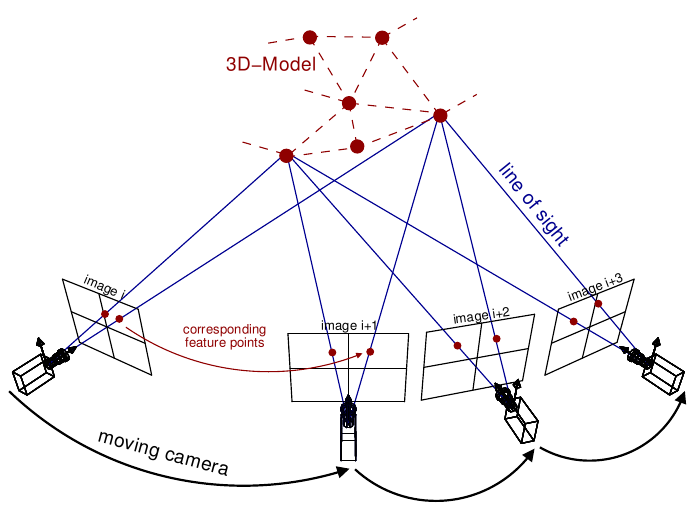
\includegraphics[scale=0.40]{Images/NubeDePuntos/StructureFromMotion(SFM).png}
    \caption[Representación de \textit{Structure From Motion (SfM)}]{Representación de \textit{Structure From Motion (SfM)}.}
    \label{fig:SFM}
\end{figure} 

Una vez comprendido a alto nivel como funciona la telemetría, ahora se profundizará un poco más dentro de este apartado.\\

Como muestra la (figura \ref{fig:Trigonometry}), se seguirán unas reglas básicas trigonométricas para resolver la posición de un único punto en el mundo real. \\

Suponiendo, por ejemplo, que se desea conocer la posición del punto A de la (figura \ref{fig:Trigonometry}), y nuestro dispositivo se encuentra en la posición B de la misma figura.
En este punto, sólo conocemos la posición y rotación de nuestro dispositivo.
Ahora realizamos un movimiento desde la posición B a la posición C. En este punto, gracias a las mediciones del dispositivo, conocemos la nueva posición y rotación (C, \textgamma), y por tanto la distancia que une a estas dos posiciones ($\overline{\mbox{#AC}}$)  que en la figura se representa por a.

Una vez se tenga tanto la posición B y C, y como sabemos la rotación del dispositivo mediante el giróscopo del mismo, tenemos los ángulos \textbeta, \textgamma. Teniendo estos dos ángulos y dado que los ángulos de cualquier triángulo han de formar 180º, también tenemos \textalpha:

$$\alpha=180º-\gamma-\beta$$

Finalmente, conocidos todos estos datos y mediante el Teorema del seno, se puede conocer tanto la distancia desde $\overline{AB}$ como $\overline{AC}$, y por consiguiente el punto A que se situará dentro de la aplicación:

$$\frac{Sen(\gamma)}{\overline{AB}}=\frac{Sen(\alpha)}{\overline{CB}} \Rightarrow \overline{AB} $$ 

$$\frac{Sen(\beta)}{\overline{AC}}=\frac{Sen(\alpha)}{\overline{CB}} \Rightarrow \overline{AC} $$ \\ \\ \\ \\

\begin{figure}[h]
    \centering
    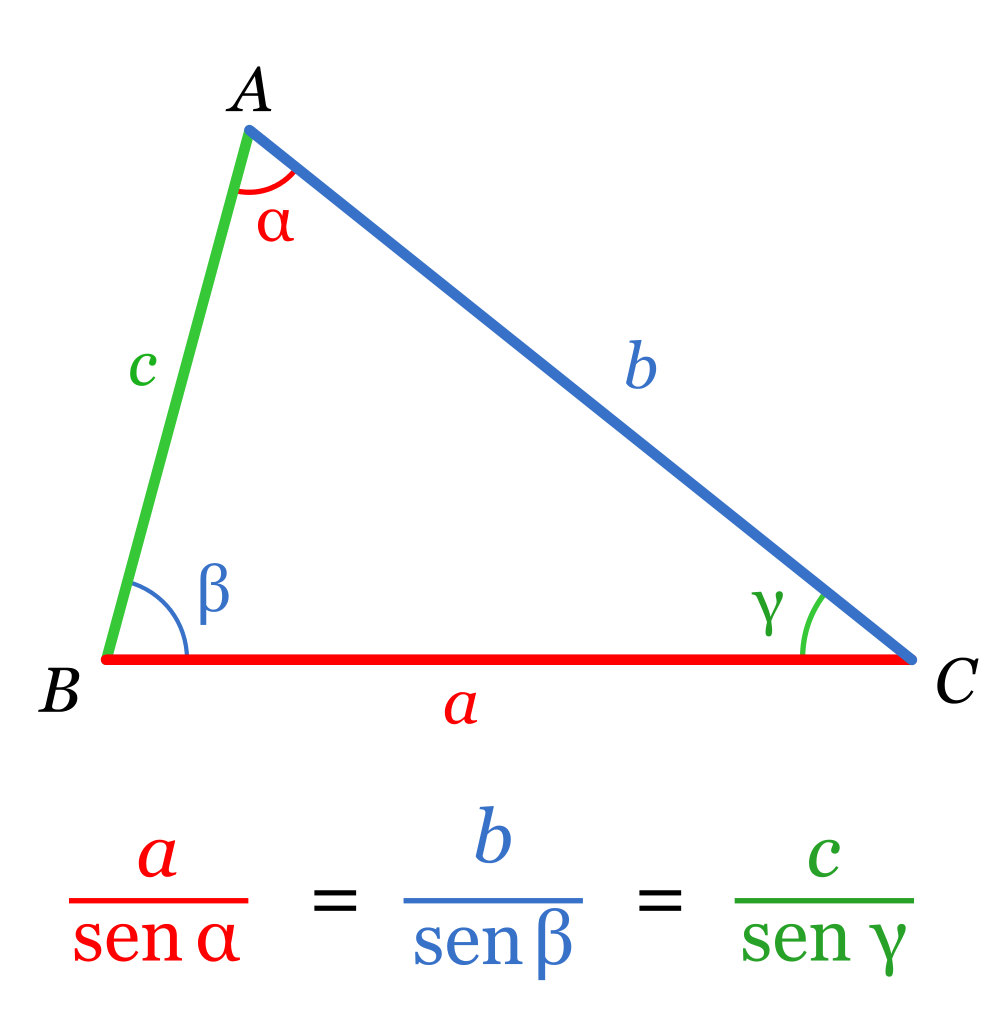
\includegraphics[scale=0.15]{Images/NubeDePuntos/Trigonometria.png}
    \caption[Principio trigonométrico para calcular distancias]{Principio trigonométrico para calcular distancias.}
    \label{fig:Trigonometry}
\end{figure}

Una vez obtengamos el punto A, sólo habrá que repetir el proceso tantas veces como \textit{``features''} haya dentro de la imagen y en consecuencia construir la nube de puntos. \\

Cuando toda la información de estos puntos esté disponible, existen varias maneras de tratarlos. Para nuestro estudio realizamos distintas pruebas aunque existen otras muchas formas de dar uso a esta nube de puntos, como la creación de una malla tridimensional para generar oclusión o simplemente obtener la información de dichos puntos para construir un objeto en tres dimensiones dentro de la aplicación.